%%%%%%%%%%%%%%%%%%%%%%%%%%%%%%%%%%%%%%%%%%%%%%%%%%%%%%%%%%%%%%%
%
% Welcome to writeLaTeX --- just edit your LaTeX on the left,
% and I'll compile it for you on the right. If you give
% someone the link to this page, they can edit at the same
% time. See the help menu above for more info. Enjoy!
%
%%%%%%%%%%%%%%%%%%%%%%%%%%%%%%%%%%%%%%%%%%%%%%%%%%%%%%%%%%%%%%%

% --------------------------------------------------------------
% This is all preamble stuff that you don't have to worry about.
% Head down to where it says "Start here"
% --------------------------------------------------------------
 
\documentclass[12pt]{report}
 
\usepackage[margin=1in]{geometry}
\usepackage{amsmath,amsthm,amssymb}
\usepackage{hyperref}
\usepackage[nottoc,numbib]{tocbibind}
\usepackage{graphicx}
\graphicspath{{./images/}}

\usepackage{listings}
\usepackage{xcolor}

%New colors defined below
\definecolor{codegreen}{rgb}{0,0.6,0}
\definecolor{codegray}{rgb}{0.5,0.5,0.5}
\definecolor{codepurple}{rgb}{0.58,0,0.82}
\definecolor{backcolour}{rgb}{0.95,0.95,0.92}

%Code listing style named "mystyle"
\lstdefinestyle{mystyle}{
  backgroundcolor=\color{backcolour}, commentstyle=\color{codegreen},
  keywordstyle=\color{magenta},
  numberstyle=\tiny\color{codegray},
  stringstyle=\color{codepurple},
  basicstyle=\ttfamily\footnotesize,
  breakatwhitespace=false,         
  breaklines=true,                 
  captionpos=b,                    
  keepspaces=true,                 
  numbers=left,                    
  numbersep=5pt,                  
  showspaces=false,                
  showstringspaces=false,
  showtabs=false,                  
  tabsize=2
}

%"mystyle" code listing set
\lstset{style=mystyle}

 
\newcommand{\N}{\mathbb{N}}
\newcommand{\Z}{\mathbb{Z}}
 
\newenvironment{theorem}[2][Theorem]{\begin{trivlist}
\item[\hskip \labelsep {\bfseries #1}\hskip \labelsep {\bfseries #2.}]}{\end{trivlist}}
\newenvironment{lemma}[2][Lemma]{\begin{trivlist}
\item[\hskip \labelsep {\bfseries #1}\hskip \labelsep {\bfseries #2.}]}{\end{trivlist}}
\newenvironment{exercise}[2][Exercise]{\begin{trivlist}
\item[\hskip \labelsep {\bfseries #1}\hskip \labelsep {\bfseries #2.}]}{\end{trivlist}}
\newenvironment{problem}[2][Problem]{\begin{trivlist}
\item[\hskip \labelsep {\bfseries #1}\hskip \labelsep {\bfseries #2.}]}{\end{trivlist}}
\newenvironment{question}[2][Question]{\begin{trivlist}
\item[\hskip \labelsep {\bfseries #1}\hskip \labelsep {\bfseries #2.}]}{\end{trivlist}}
\newenvironment{corollary}[2][Corollary]{\begin{trivlist}
\item[\hskip \labelsep {\bfseries #1}\hskip \labelsep {\bfseries #2.}]}{\end{trivlist}}

\newenvironment{solution}{\begin{proof}[Solution]}{\end{proof}}
 
\begin{document}
 
% --------------------------------------------------------------
%                         Start here
% --------------------------------------------------------------
 
\title{Texas A\&M University Kingsville\\
Department of EECS\\
CSEN 5303 Foundations of Computer Science\\
Project 1 Conway's Game of Life
}%Institution, Department
\author{Ameya Khot\\
Mengxiang Jiang\\ %replace with your name
Professor Habib Ammari} %if necessary, replace with your course title
 
\maketitle

\tableofcontents

\chapter{Introduction}
In 1968, John Conway, an English mathematician at Cambridge University, 
tried to simplify a machine with a set of complicated rules to replicate itself on
a 2D grid of squares by John von Neumann. He didn't use a computer to simulate his rules, but rather ``shuffled poker chips, foreign coins, 
cowrie shells, Go stones or whatever came to hand, until there was a viable balance between life and death."\cite{o'connor:2004}
When he finally succeeded, his game would remain mainly an academic curiosity until he showed it in 1970 to
Martin Gardner, a great popularizer of recreational mathematics. Gardner put the game into his
``Mathematical Games" column of \emph{Scientific American}, and it became the most popular column he had ever written as well as 
``made Conway an instant celebrity. The game was written up in \emph{Time}."\cite{mulcahy:2014} And the rest is history as the saying goes.\\\\
Well, I'm sure you're very excited to learn about the simple rules of Conway's Game of Life. And it is actually very simple. They are:

1. A live cell lives if it has two or three neighbors and dies otherwise.

2. A dead cell becomes alive if it has exactly three live neighbors, otherwise it stays dead.\\\\
Despite how simple these rules are, the complexity of the behavior of these cells is extremely difficult to predict.
In fact, this seemingly simple game has been proven to be equivalent to a universal Turing machine, which basically
means that it can be used to program any software that your favorite programming language is capable of programming 
(assuming your favorite programming language is Turing complete of course).\cite{rendell:2011}
This paper will not be delving into any depth of this complexity.\\\\
Instead, the main purpose of this paper is to explain an implementation of the game using an object oriented approach in Python,
and utilizing the Pygame library to display the cells from generation to generation. Some of the optimization ideas from
a C++ implementation by the legendary game programmer Michael Abrash in his famous \emph{Michael Abrash's Graphics Programming Black Book}.\cite{abrash:1997}

\chapter{Design}
The main data structure we used to capture the 2D grid of squares for the cells is, fairly obviously, a 2D array.
However, rather than simply use the raw 2D array, we decided to create a class wrapper around it called \emph{cellmap}.
There are two main advantages to this. One, higher level users do not need to know the implementation details and can treat
it as a black box, so if a more efficient data structure or implementation is found, 
the higher level users will not need to change their code.
Two, some of the functionality should not be modified by higher level users, so using a wrapper class allows us to encapsulate the functionality I want private.
The basic functionality of a $cellmap$ object is detailed below:
\begin{verbatim}
class cellmap
    private width
    private height
    private cells
    private changed
    private generation
    private steady state

    public procedure new(width, height, rand, file)
        // initialize variables of the cellmap 
        // if rand is true, randomly assign cells as live or dead
        // if file is present, use file to assign cells
    endprocedure

    private procedure turn_cell_on(x, y)
        // sets the state of the cell at coord (x, y) to be alive
    endprocedure

    private procedure turn_cell_off(x, y)
        // sets the state of the cell at coord (x, y) to be dead
    endprocedure

    private procedure count_on_neighbors(x, y)
        // counts live neighbors of the cell at coord (x, y)
    endprocedure

    public procedure cell_state(x, y)
        // returns the state of the cell at coord (x, y)
        // if (x, y) is out of bounds return dead
    endprocedure

    public procedure next_generation()
        // evaluates the next generation of cells in a new cellmap
        // returns the new cellmap if at least one cell changed
    endprocedure

    public procedure write_to_file(file)
        // write the states of the cell to the given file
        // used for testing/debugging purposes
    endprocedure

endclass
\end{verbatim}
Most of the functionality is very trivial, so we will go over the two parts that are slightly more complex,
namely the \emph{count\_on\_neighbors} and \emph{next\_generation}:\\

For \emph{count\_on\_neighbors}, rather than use three different cases (cells at the corners, edges, and center), we generalized
the cases to just consider all cells as if they were in the center and therefore always having 8 neighbors. 
There are two ways to do this, one as stated in class is the pad the 2D array on the outside with dead cells.
The other, which is the way we did it here, is to have the getter method (\emph{cell\_state}), return the state of 
out of bounds cells as dead.\\

For \emph{next\_generation}, first the old $cellmap$ has its private variable $steady\_state$ checked.
If it's true, then it simply returns the old $cellmap$ since it has reached steady state.
Else, a new $cellmap$ is allocated, each cell of the old $cellmap$ has its neighbors counted.
This count determined whether the corresponding cell in the new $cellmap$ lives or dies, based on the rules. 
Whenever a new cell state changes (from live to dead or vice versa), it is added to the $changed$ stack of the new $cellmap$ 
($changed$ is initialized to be empty on every newly constructed $cellmap$).
If $changed$ is empty at the end of checking all the old cells, the old $cellmap$ changes the $steady\_state$ to true and returns
itself. Otherwise, the new $cellmap$ has the $generation$ counter incremented by one, and is returned.\\\\
This is all well and good, but how do we view the $cellmap$ and successive generations of it?
Well, we need some form of drawing/displaying of the cells on a continuous loop, and this sounds very much like a game engine.
It just so happens that Python has a fairly decent game engine library called Pygame, which we imported rather than implement our own from scratch.\cite{pygame}

\chapter{Code}
\begin{lstlisting}[language=Python, caption=cell\_map.py]
"""
cell map class for keeping track of cells for game of life
"""
# Import random library since I need to randomly generate a cell map at the start
import random

class cellmap:
    ADJACENT = [[-1, -1], [-1, 0], [-1, 1], [0, -1], [0, 1], [1, -1], [1, 0], [1, 1]]

    # cellmap constructor
    def __init__(self, width, height, rand=False, file=None):
        self.width = width
        self.height = height
        self.cells = [[0]*self.height for i in range(self.width)]
        self.changed = []
        self.generation = 0
        self.steady_state = False
        if rand:
            for x in range(width):
                for y in range(height):
                    if random.random() > 0.5:
                        self.turn_cell_on(x, y)
        if file:
            f = open(file, 'r')
            self.width = int(f.readline())
            self.height = int(f.readline())
            self.cells = [[0]*self.height for i in range(self.width)]
            for y in range(self.height):
                for x, c in enumerate(f.readline()):
                    if c == '0':
                        self.turn_cell_off(x, y)
                    if c == '1':
                        self.turn_cell_on(x, y)
            f.close()
    
    # writes cellmap to file
    def write_to_file(self, file):
        f = open(file, 'w')
        f.writelines([f'{self.width}', '\n', f'{self.height}', '\n'])
        for y in range(self.height):
            for x in range(self.width):
                f.write(str(self.cell_state(x, y)))
            f.write('\n')
        f.close()

    # turns cell on
    def turn_cell_on(self, x, y):
        self.cells[x][y] = 1
    
    # turns cell off
    def turn_cell_off(self, x, y):
        self.cells[x][y] = 0

    # returns the cell state
    def cell_state(self, x, y):
        if 0 <= x < self.width and 0 <= y < self.height:
            return self.cells[x][y]
        else:
            return 0
    
    # count the number of neighbors on of a given cell
    def count_on_neighbors(self, x, y):
        neighbor_count = 0
        for i, j in self.ADJACENT:
            neighbor_count += self.cell_state(x + i, y + j)
        return neighbor_count

    # returns the next generation cell map
    def next_generation(self):
        if self.steady_state:
            return self
        else:
            next_map = cellmap(self.width, self.height)

            for x in range(self.width):
                for y in range(self.height):
                    neighbor_count = self.count_on_neighbors(x, y)
                    # if the cell is on, turn it off if it has too many or too few on neighbors
                    if self.cell_state(x, y):
                        if neighbor_count < 2 or neighbor_count > 3:
                            next_map.turn_cell_off(x, y)
                            next_map.changed.append((x, y))
                        else:
                            next_map.turn_cell_on(x, y)
                    # if the cell is off, turn it on if it has enough on neighbors
                    else:
                        if neighbor_count == 3:
                            next_map.turn_cell_on(x, y)
                            next_map.changed.append((x, y))
            if len(next_map.changed) == 0:
                self.steady_state = True
                return self
            else:
                next_map.generation = self.generation + 1
                return next_map
\end{lstlisting}

\begin{lstlisting}[language=Python, caption=game\_of\_life.py]
# https://www.jagregory.com/abrash-black-book/#chapter-17-the-game-of-life

"""
Basic Game of Life program in Python using the Pygame library to draw
"""

# Import libraries
from email import message
from tkinter import filedialog
import pygame
import pygame_menu
import random
from cell_map import cellmap
from tkinter import *
from tkinter import messagebox
import win32gui

root = Tk()
root.wm_withdraw() #to hide the main window

pygame.init()

# font for pygame
pygame_font = pygame.font.Font('WHITRABT.ttf', 30)

# States of the game:
MAIN_MENU = 0
PLAYING = 1

# Window constants
WINDOW_WIDTH = 800
WINDOW_HEIGHT = 600

# Text constants
WIDTH_TEXT_X = 520
WIDTH_TEXT_Y = 50
HEIGHT_TEXT_X = 520
HEIGHT_TEXT_Y = 100
GENERATION_TEXT_X = 520
GENERATION_TEXT_Y = 150
LIVE_TEXT_X = 520
LIVE_TEXT_Y = 200
DEAD_TEXT_X = 520
DEAD_TEXT_Y = 250
STEADY_TEXT_X = 520
STEADY_TEXT_Y = 300
TEXT_COLOR = (200, 200, 200)

# Button constants
BUTTON_WIDTH_LARGE = 200
BUTTON_WIDTH_SMALL = 100
BUTTON_HEIGHT = 50
NEXT_BUTTON_X = 50
NEXT_BUTTON_Y = 520
AUTO_BUTTON_X = 200
AUTO_BUTTON_Y = 520
WRITE_BUTTON_X = 450
WRITE_BUTTON_Y = 520
BACK_BUTTON_X = 600
BACK_BUTTON_Y = 520
BUTTON_LIGHT = (170, 170, 170)
BUTTON_DARK = (100, 100, 100)
BUTTON_TEXT_COLOR = (0, 255, 0)
BUTTON_TEXT_OFFSET_X = 10
BUTTON_TEXT_OFFSET_Y = 10

# Initial state should be on the main menu
game_state = MAIN_MENU

# How quickly should the next generation be created? Time in milliseconds
GEN_INTERVAL = 100

# Create a custom event for next cell generation
NEXTGEN = pygame.USEREVENT + 1
pygame.time.set_timer(NEXTGEN, GEN_INTERVAL)

# cell map displaying variables
cellmap_width = random.randint(1, 100)
cellmap_height = random.randint(1, 100)
cell_pixel_size = 4

# cell colors (Official Blue and Gold from TAMUK graphics standards)
# https://www.tamuk.edu/marcomm/_images_MARCOMM/branding/graphic_standards.pdf
live_color = (255, 196, 37)
dead_color = (0, 93, 170)

# Set up the drawing window
screen = pygame.display.set_mode((WINDOW_WIDTH, WINDOW_HEIGHT))
pygame.display.set_caption('Game of Life')

# generates a random cell map
current_map = cellmap(cellmap_width, cellmap_height, rand=True)

# writing the current_map to a file for debugging purposes
current_map.write_to_file('current_map.txt')

about_menu = pygame_menu.Menu('About', WINDOW_WIDTH, WINDOW_HEIGHT,
                        theme=pygame_menu.themes.THEME_DARK)
about_menu.add.label('This is a programming project for the course')
about_menu.add.label('Foundations of Computer Science at TAMUK.')
about_menu.add.label('The Game of Life is a 2D simulation of cells')
about_menu.add.label('that live or die in successive generations.')
about_menu.add.label('Only the starting state of the cells is needed')
about_menu.add.label('to produce the next generation, so this is not')
about_menu.add.label('very interactive beyond setting initial conditions.')
about_menu.add.label('The authors are Ameya Khot and Mengxiang Jiang.')

about_menu.add.label('')
about_menu.add.button('Back', pygame_menu.events.BACK)

settings_menu = pygame_menu.Menu('Settings', WINDOW_WIDTH, WINDOW_HEIGHT,
                        theme=pygame_menu.themes.THEME_DARK)
def check_cellmap_width(value):
    global cellmap_width
    if value < 0:
        messagebox.showerror('Invalid width', 'value must be positive')
    elif value > 100:
        messagebox.showerror('Invalid width', 'value must be less than 100')
    else:
        cellmap_width = value

settings_menu.add.text_input(
    'Width: ',
    default=cellmap_width,
    onchange=check_cellmap_width,
    input_type=pygame_menu.locals.INPUT_INT,
    textinput_id='cellmap_width'
)

def check_cellmap_height(value):
    global cellmap_height
    if value < 0:
        messagebox.showerror('Invalid height', 'value must be positive')
    elif value > 100:
        messagebox.showerror('Invalid height', 'value must be less than 100')
    else:
        cellmap_height = value

settings_menu.add.text_input(
    'Height: ',
    default=cellmap_height,
    onchange=check_cellmap_height,
    input_type=pygame_menu.locals.INPUT_INT,
    textinput_id='cellmap_height'
)

def check_live_color(value):
    global live_color
    global dead_color
    if value == dead_color:
        messagebox.showerror('Invalid live color', 'color must be different from dead color')
    else:
        live_color = value

settings_menu.add.color_input(
    'Live Color (R,G,B): ',
    default=live_color,
    color_type=pygame_menu.widgets.COLORINPUT_TYPE_RGB,
    onchange=check_live_color,
    color_id='live_color'
    )

def check_dead_color(value):
    global live_color
    global dead_color
    if value == live_color:
        messagebox.showerror('Invalid dead color', 'color must be different from livecolor')
    else:
        dead_color = value

settings_menu.add.color_input(
    'Dead Color (R,G,B): ',
    default=dead_color,
    color_type=pygame_menu.widgets.COLORINPUT_TYPE_RGB,
    onchange=check_dead_color,
    color_id='dead_color'
    )

def load_from_file():
    f = filedialog.askopenfilename()
    hwnd = pygame.display.get_wm_info()['window']
    win32gui.SetFocus(hwnd)
    start_the_game()
    global current_map
    global cellmap_width
    global cellmap_height
    current_map = cellmap(cellmap_width, cellmap_height, file=f)
    cellmap_width = current_map.width
    cellmap_height = current_map.height

settings_menu.add.button('Load from file', load_from_file)

settings_menu.add.button('Back', pygame_menu.events.BACK)

main_menu = pygame_menu.Menu('Conway\'s Game of Life', WINDOW_WIDTH, WINDOW_HEIGHT,
                        theme=pygame_menu.themes.THEME_DARK)

def start_the_game():
    global game_state
    global main_menu
    global current_map
    global cellmap_width
    global cellmap_height
    game_state = PLAYING
    main_menu.disable()
    screen.fill((0, 0, 0))
    current_map = cellmap(cellmap_width, cellmap_height, rand=True)

main_menu.add.button('Play', start_the_game)
main_menu.add.button('About', about_menu)  # Add about submenu
main_menu.add.button('Settings', settings_menu) # Add settings submenu
main_menu.add.button('Quit', pygame_menu.events.EXIT)


# state for checking whether the user wants the next generation to be generated automatically
auto_state = False

def draw_next_button(mouse):
    if NEXT_BUTTON_X <= mouse[0] <= (NEXT_BUTTON_X + BUTTON_WIDTH_SMALL) \
    and NEXT_BUTTON_Y <= mouse[1] <= (NEXT_BUTTON_Y + BUTTON_HEIGHT):
        pygame.draw.rect(screen, BUTTON_LIGHT, [NEXT_BUTTON_X, NEXT_BUTTON_Y, BUTTON_WIDTH_SMALL, BUTTON_HEIGHT])
    else:
        pygame.draw.rect(screen, BUTTON_DARK, [NEXT_BUTTON_X, NEXT_BUTTON_Y, BUTTON_WIDTH_SMALL, BUTTON_HEIGHT])
    text = pygame_font.render('NEXT', True, BUTTON_TEXT_COLOR)
    screen.blit(text, (NEXT_BUTTON_X + BUTTON_TEXT_OFFSET_X, NEXT_BUTTON_Y + BUTTON_TEXT_OFFSET_Y))

def draw_auto_button(mouse):
    if AUTO_BUTTON_X <= mouse[0] <= (AUTO_BUTTON_X + BUTTON_WIDTH_LARGE) \
    and AUTO_BUTTON_Y <= mouse[1] <= (AUTO_BUTTON_Y + BUTTON_HEIGHT):
        pygame.draw.rect(screen, BUTTON_LIGHT, [AUTO_BUTTON_X, AUTO_BUTTON_Y, BUTTON_WIDTH_LARGE, BUTTON_HEIGHT])
    else:
        pygame.draw.rect(screen, BUTTON_DARK, [AUTO_BUTTON_X, AUTO_BUTTON_Y, BUTTON_WIDTH_LARGE, BUTTON_HEIGHT])
    text = pygame_font.render(f'AUTO: {auto_state}', True, BUTTON_TEXT_COLOR)
    screen.blit(text, (AUTO_BUTTON_X + BUTTON_TEXT_OFFSET_X, AUTO_BUTTON_Y + BUTTON_TEXT_OFFSET_Y))

def draw_write_button(mouse):
    if WRITE_BUTTON_X <= mouse[0] <= (WRITE_BUTTON_X + BUTTON_WIDTH_SMALL) \
    and WRITE_BUTTON_Y <= mouse[1] <= (WRITE_BUTTON_Y + BUTTON_HEIGHT):
        pygame.draw.rect(screen, BUTTON_LIGHT, [WRITE_BUTTON_X, WRITE_BUTTON_Y, BUTTON_WIDTH_SMALL, BUTTON_HEIGHT])
    else:
        pygame.draw.rect(screen, BUTTON_DARK, [WRITE_BUTTON_X, WRITE_BUTTON_Y, BUTTON_WIDTH_SMALL, BUTTON_HEIGHT])
    text = pygame_font.render('WRITE', True, BUTTON_TEXT_COLOR)
    screen.blit(text, (WRITE_BUTTON_X + BUTTON_TEXT_OFFSET_X, WRITE_BUTTON_Y + BUTTON_TEXT_OFFSET_Y))

def draw_back_button(mouse):
    if BACK_BUTTON_X <= mouse[0] <= (BACK_BUTTON_X + BUTTON_WIDTH_SMALL) \
    and BACK_BUTTON_Y <= mouse[1] <= (BACK_BUTTON_Y + BUTTON_HEIGHT):
        pygame.draw.rect(screen, BUTTON_LIGHT, [BACK_BUTTON_X, BACK_BUTTON_Y, BUTTON_WIDTH_SMALL, BUTTON_HEIGHT])
    else:
        pygame.draw.rect(screen, BUTTON_DARK, [BACK_BUTTON_X, BACK_BUTTON_Y, BUTTON_WIDTH_SMALL, BUTTON_HEIGHT])
    text = pygame_font.render('BACK', True, BUTTON_TEXT_COLOR)
    screen.blit(text, (BACK_BUTTON_X + BUTTON_TEXT_OFFSET_X, BACK_BUTTON_Y + BUTTON_TEXT_OFFSET_Y))

def draw_width_text():
    text = pygame_font.render(f'Width: {cellmap_width}', True, TEXT_COLOR)
    screen.blit(text, (WIDTH_TEXT_X, WIDTH_TEXT_Y))

def draw_height_text():
    text = pygame_font.render(f'Height: {cellmap_height}', True, TEXT_COLOR)
    screen.blit(text, (HEIGHT_TEXT_X, HEIGHT_TEXT_Y))

def draw_generation_text():
    text = pygame_font.render(f'Generation: {current_map.generation}', True, TEXT_COLOR)
    screen.fill((0, 0, 0), [GENERATION_TEXT_X, GENERATION_TEXT_Y, 300, 300])
    screen.blit(text, (GENERATION_TEXT_X, GENERATION_TEXT_Y))

def draw_live_color():
    text = pygame_font.render('Live Color: ', True, TEXT_COLOR)
    pygame.draw.rect(screen, live_color, [LIVE_TEXT_X + 200, LIVE_TEXT_Y, 20, 20])
    screen.blit(text, (LIVE_TEXT_X, LIVE_TEXT_Y))

def draw_dead_color():
    text = pygame_font.render('Dead Color: ', True, TEXT_COLOR)
    pygame.draw.rect(screen, dead_color, [DEAD_TEXT_X + 200, DEAD_TEXT_Y, 20, 20])
    screen.blit(text, (DEAD_TEXT_X, DEAD_TEXT_Y))

def draw_steady_state():
    text = pygame_font.render(f'Finished: {current_map.steady_state}', True, TEXT_COLOR)
    screen.fill((0, 0, 0), [STEADY_TEXT_X, STEADY_TEXT_Y, 300, 100])
    screen.blit(text, (STEADY_TEXT_X, STEADY_TEXT_Y))

# Run until the user asks to quit
running = True
while running:
    # gets the current mouse position
    mouse = pygame.mouse.get_pos()

    # Did the user click the window close button?
    for event in pygame.event.get():
        if event.type == pygame.QUIT:
            running = False

        # Should the next generation be displayed?
        elif event.type == NEXTGEN:
            if game_state == PLAYING and auto_state:
                current_map = current_map.next_generation()
                # Stop the previous timer by setting the interval to 0
                pygame.time.set_timer(NEXTGEN, 0)
                # Start a new timer
                pygame.time.set_timer(NEXTGEN, GEN_INTERVAL)
        elif event.type == pygame.MOUSEBUTTONDOWN:
            if game_state == PLAYING:
                if NEXT_BUTTON_X <= mouse[0] <= (NEXT_BUTTON_X + BUTTON_WIDTH_SMALL) \
                    and NEXT_BUTTON_Y <= mouse[1] <= (NEXT_BUTTON_Y + BUTTON_HEIGHT):
                    current_map = current_map.next_generation()
                elif AUTO_BUTTON_X <= mouse[0] <= (AUTO_BUTTON_X + BUTTON_WIDTH_LARGE) \
                    and AUTO_BUTTON_Y <= mouse[1] <= (AUTO_BUTTON_Y + BUTTON_HEIGHT):
                    auto_state = not auto_state
                elif WRITE_BUTTON_X <= mouse[0] <= (WRITE_BUTTON_X + BUTTON_WIDTH_SMALL) \
                    and WRITE_BUTTON_Y <= mouse[1] <= (WRITE_BUTTON_Y + BUTTON_HEIGHT):
                    f = filedialog.askopenfilename()
                    hwnd = pygame.display.get_wm_info()['window']
                    win32gui.SetFocus(hwnd)
                    current_map.write_to_file(f)
                elif BACK_BUTTON_X <= mouse[0] <= (BACK_BUTTON_X + BUTTON_WIDTH_SMALL) \
                    and BACK_BUTTON_Y <= mouse[1] <= (BACK_BUTTON_Y + BUTTON_HEIGHT):
                    game_state = MAIN_MENU
                    main_menu.enable()

    if game_state == MAIN_MENU:
        main_menu.mainloop(screen)

    if game_state == PLAYING:
        draw_next_button(mouse)
        draw_auto_button(mouse)
        draw_write_button(mouse)
        draw_back_button(mouse)
        draw_width_text()
        draw_height_text()
        draw_generation_text()
        draw_live_color()
        draw_dead_color()
        draw_steady_state()

        # Check every cell of the entire cell map if it's the first 10 iterations
        if current_map.generation == 0:
            for x in range(current_map.width):
                for y in range(current_map.height):
                    if current_map.cell_state(x, y):
                        pygame.draw.rect(screen, live_color, 
                        [(cell_pixel_size + 1) * (x + 1), (cell_pixel_size + 1) * (y + 1), cell_pixel_size, cell_pixel_size])
                    else:
                        pygame.draw.rect(screen, dead_color, 
                        [(cell_pixel_size + 1) * (x + 1), (cell_pixel_size + 1) * (y + 1), cell_pixel_size, cell_pixel_size])
        # Else only draw cells that have changed
        else:
            for x, y in current_map.changed:
                if current_map.cell_state(x, y):
                    pygame.draw.rect(screen, live_color, 
                    [(cell_pixel_size + 1) * (x + 1), (cell_pixel_size + 1) * (y + 1), cell_pixel_size, cell_pixel_size])
                else:
                    pygame.draw.rect(screen, dead_color, 
                    [(cell_pixel_size + 1) * (x + 1), (cell_pixel_size + 1) * (y + 1), cell_pixel_size, cell_pixel_size])

    # Flip the display to make everything appear
    pygame.display.flip()

# Done! Time to quit.
pygame.quit()

\end{lstlisting}

\begin{figure}[h]
    \centering
    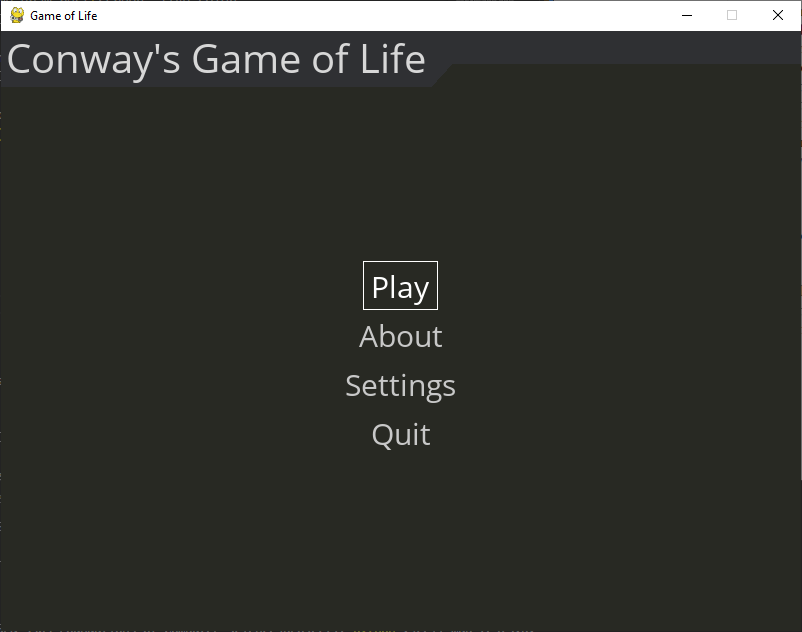
\includegraphics[width=\textwidth]{mainmenu}
    \caption{main menu}
\end{figure}

\begin{figure}[h]
    \centering
    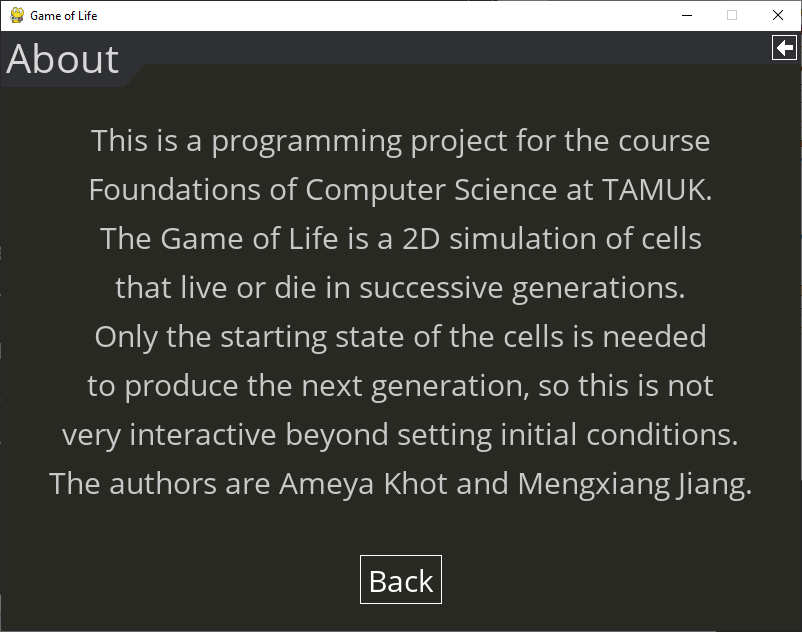
\includegraphics[width=\textwidth]{about}
    \caption{about}
\end{figure}

\begin{figure}[h]
    \centering
    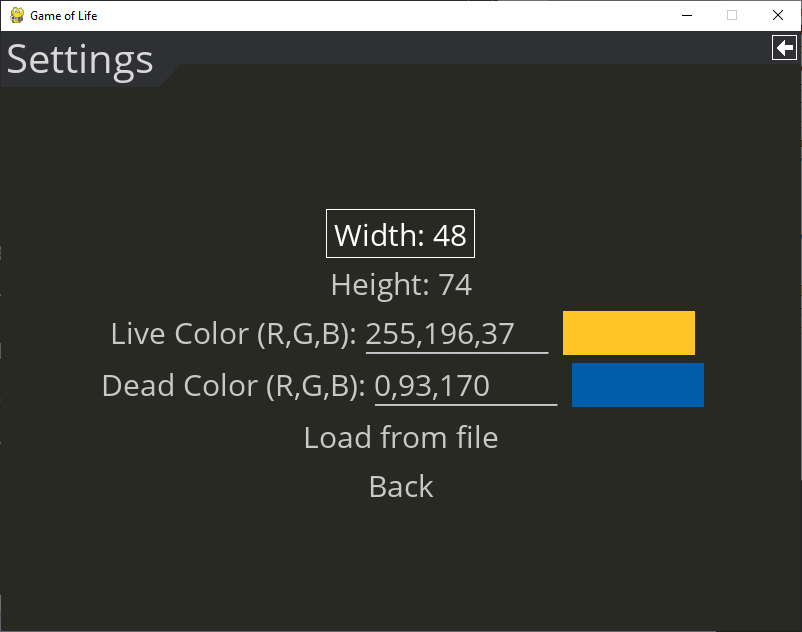
\includegraphics[width=\textwidth]{settings}
    \caption{settings}
\end{figure}

\begin{figure}[h]
    \centering
    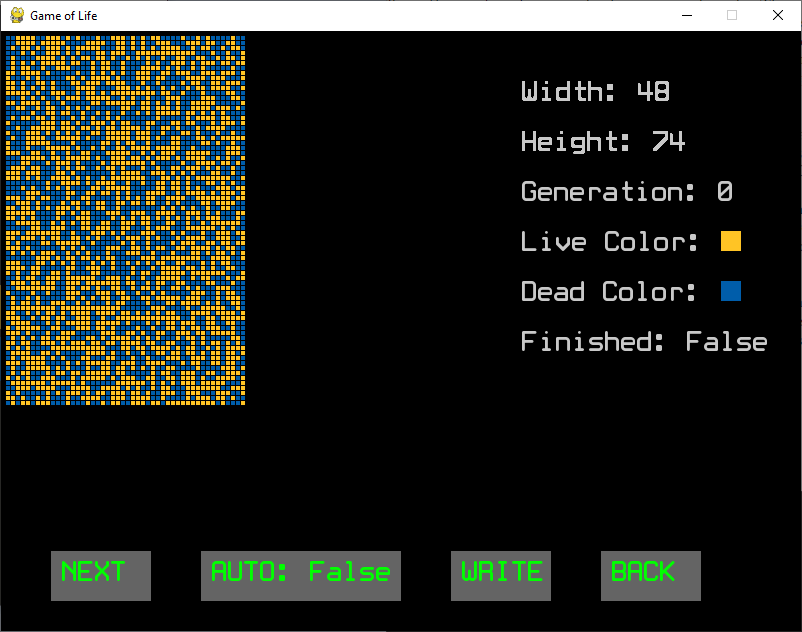
\includegraphics[width=\textwidth]{play}
    \caption{playing}
\end{figure}

\chapter{Tests}

\begin{lstlisting}[language=Python, caption=cell\_map\_tests.py]
import unittest
import filecmp
from cell_map import cellmap

class TestCellMap(unittest.TestCase):
    # empty cellmap will not change in the next generation
    def test_empty(self):
        current_map = cellmap(3, 3, file='tests/empty.txt')
        next_map = current_map.next_generation()
        next_map.write_to_file('tests/next.txt')
        self.assertTrue(filecmp.cmp('tests/empty.txt', 'tests/next.txt'))
    
    # cellmap with a 2x2 square will not change in the next generation
    def test_square(self):
        current_map = cellmap(3, 3, file='tests/square.txt')
        next_map = current_map.next_generation()
        next_map.write_to_file('tests/next.txt')
        self.assertTrue(filecmp.cmp('tests/square.txt', 'tests/next.txt'))

    # cellmap with a 1x3 horizontal line will change to a 3x1 vertical line
    def test_horizontal(self):
        current_map = cellmap(3, 3, file='tests/horizontal.txt')
        next_map = current_map.next_generation()
        next_map.write_to_file('tests/next.txt')
        self.assertTrue(filecmp.cmp('tests/vertical.txt', 'tests/next.txt'))

    # cellmap with a 3x1 vertical line will change to a 1x3 horizontal line
    def test_vertical(self):
        current_map = cellmap(3, 3, file='tests/vertical.txt')
        next_map = current_map.next_generation()
        next_map.write_to_file('tests/next.txt')
        self.assertTrue(filecmp.cmp('tests/horizontal.txt', 'tests/next.txt'))

    # a glider in the top left corner of a 5x5 matrix
    # will glide down to the bottom right corner and become a square
    def test_glider(self):
        current_map = cellmap(5,5, file='tests/glider0.txt')
        next_map = current_map.next_generation()
        next_map.write_to_file('tests/next.txt')
        for i in range(1, 11):
            self.assertTrue(filecmp.cmp(f'tests/glider{i}.txt', 'tests/next.txt'))
            next_map = next_map.next_generation()
            next_map.write_to_file('tests/next.txt')
        self.assertTrue(filecmp.cmp('tests/square2.txt', 'tests/next.txt'))

unittest.main()
\end{lstlisting}

\begin{lstlisting}[language=Python, caption=empty.txt]
3
3
000
000
000
\end{lstlisting}

\begin{lstlisting}[language=Python, caption=glider0.txt]
5
5
01000
00100
11100
00000
00000
\end{lstlisting}

\begin{lstlisting}[language=Python, caption=glider1.txt]
5
5
00000
10100
01100
01000
00000
\end{lstlisting}

\begin{lstlisting}[language=Python, caption=glider2.txt]
5
5
00000
00100
10100
01100
00000
\end{lstlisting}

glider3 to glider10 omitted for brevity

\begin{lstlisting}[language=Python, caption=horizontal.txt]
3
3
000
111
000
\end{lstlisting}

\begin{lstlisting}[language=Python, caption=square.txt]
3
3
000
110
110
\end{lstlisting}

\begin{lstlisting}[language=Python, caption=square2.txt]
5
5
00000
00000
00000
00011
00011
\end{lstlisting}

\begin{lstlisting}[language=Python, caption=vertical.txt]
3
3
010
010
010
\end{lstlisting}



\chapter{Lessons Learned}
The logic for evaluating the game is very simple and straightforward to implement. 
However, for large grid sizes, it becomes very slow very quickly, since the number of cells grows quadratically as the number of rows and columns grows linearly.
There are actually quite a large number of optimizations, many of them detailed in \emph{Michael Abrash's Graphics Programming Black Book}, but many of the ones listed there 
are specialized for assembly and/or specialized memory access, which unfortunately is either very difficult or impossible to do in Python.\cite{abrash:1997} One of the optimizations I did implement, however,
was keeping track of what cells changed and only drawing those rather than drawing every cell every generation. Keeping track of the changed cells also came in handy when I needed to figure out
when the cells reached steady state, since that only happens when the number of changed cells becomes 0. Back to the lesson learned, 
I guess the big lesson here is that if I want to write a very optimized game of life, I would need to write it in a lower level language like C, C++, Rust, etc.\\\\
The second big lesson I learned was that the presentation and user interface is as hard if not harder than the core logic and evaluation code of the game.
Creating the menus, buttons, and colors look half decent took about five times the effort and time as the core logic.\\\\
The third lesson was that I learned a lot of new ways to do things, since it was my first time using Pygame and the Python unit testing framework. 
I also haven't written a long report in \LaTeX, so learning how to do bibliography and table of contents was pretty cool.
\bibliographystyle{plain}
\bibliography{refs.bib}

% --------------------------------------------------------------
%     You don't have to mess with anything below this line.
% --------------------------------------------------------------
 
\end{document}